% Options for packages loaded elsewhere
\PassOptionsToPackage{unicode}{hyperref}
\PassOptionsToPackage{hyphens}{url}
\PassOptionsToPackage{dvipsnames,svgnames*,x11names*}{xcolor}
%
\documentclass[
]{article}
\usepackage{lmodern}
\usepackage{amssymb,amsmath}
\usepackage{ifxetex,ifluatex}
\ifnum 0\ifxetex 1\fi\ifluatex 1\fi=0 % if pdftex
  \usepackage[T1]{fontenc}
  \usepackage[utf8]{inputenc}
  \usepackage{textcomp} % provide euro and other symbols
\else % if luatex or xetex
  \usepackage{unicode-math}
  \defaultfontfeatures{Scale=MatchLowercase}
  \defaultfontfeatures[\rmfamily]{Ligatures=TeX,Scale=1}
\fi
% Use upquote if available, for straight quotes in verbatim environments
\IfFileExists{upquote.sty}{\usepackage{upquote}}{}
\IfFileExists{microtype.sty}{% use microtype if available
  \usepackage[]{microtype}
  \UseMicrotypeSet[protrusion]{basicmath} % disable protrusion for tt fonts
}{}
\makeatletter
\@ifundefined{KOMAClassName}{% if non-KOMA class
  \IfFileExists{parskip.sty}{%
    \usepackage{parskip}
  }{% else
    \setlength{\parindent}{0pt}
    \setlength{\parskip}{6pt plus 2pt minus 1pt}}
}{% if KOMA class
  \KOMAoptions{parskip=half}}
\makeatother
\usepackage{xcolor}
\IfFileExists{xurl.sty}{\usepackage{xurl}}{} % add URL line breaks if available
\IfFileExists{bookmark.sty}{\usepackage{bookmark}}{\usepackage{hyperref}}
\hypersetup{
  pdftitle={Political news coverage of massmedia},
  pdfauthor={Franziska Löw},
  colorlinks=true,
  linkcolor=blue,
  filecolor=Maroon,
  citecolor=Blue,
  urlcolor=Blue,
  pdfcreator={LaTeX via pandoc}}
\urlstyle{same} % disable monospaced font for URLs
\usepackage[margin=1in]{geometry}
\usepackage{longtable,booktabs}
% Correct order of tables after \paragraph or \subparagraph
\usepackage{etoolbox}
\makeatletter
\patchcmd\longtable{\par}{\if@noskipsec\mbox{}\fi\par}{}{}
\makeatother
% Allow footnotes in longtable head/foot
\IfFileExists{footnotehyper.sty}{\usepackage{footnotehyper}}{\usepackage{footnote}}
\makesavenoteenv{longtable}
\usepackage{graphicx,grffile}
\makeatletter
\def\maxwidth{\ifdim\Gin@nat@width>\linewidth\linewidth\else\Gin@nat@width\fi}
\def\maxheight{\ifdim\Gin@nat@height>\textheight\textheight\else\Gin@nat@height\fi}
\makeatother
% Scale images if necessary, so that they will not overflow the page
% margins by default, and it is still possible to overwrite the defaults
% using explicit options in \includegraphics[width, height, ...]{}
\setkeys{Gin}{width=\maxwidth,height=\maxheight,keepaspectratio}
% Set default figure placement to htbp
\makeatletter
\def\fps@figure{htbp}
\makeatother
\setlength{\emergencystretch}{3em} % prevent overfull lines
\providecommand{\tightlist}{%
  \setlength{\itemsep}{0pt}\setlength{\parskip}{0pt}}
\setcounter{secnumdepth}{-\maxdimen} % remove section numbering

\title{Political news coverage of massmedia}
\usepackage{etoolbox}
\makeatletter
\providecommand{\subtitle}[1]{% add subtitle to \maketitle
  \apptocmd{\@title}{\par {\large #1 \par}}{}{}
}
\makeatother
\subtitle{\ldots{}}
\author{Franziska Löw\footnote{Institut für Industrieökonomik, Helmut Schmidt
  Universität. Email: .}}
\date{November 2020}

\begin{document}
\maketitle

\hypertarget{introduction}{%
\section{Introduction}\label{introduction}}

In democracies, the media fulfill fundamental functions: They should
inform the people, contribute to the formation of opinion through
criticism and discussion and thus enable participation. In recent
decades, however, concern has grown about the role of the media in
politics in general and in election campaigns in particular. They are
criticized for influencing election results through their reporting and
for helping populist parties in particular to flourish. After the 2017
federal elections in Germany, for example, the media were accused of
contributing to the success of the right-wing populist AfD by
increasingly including the party's content and using the same language
in their articles as the AfD. Representatives of these media houses
strongly opposed this accusation. The purpose of this study is to
examine whether there is evidence that support the accusation of biased
media reporting, especially during election campaigns.

For advertising-financed media the battle for the attention of the
recipients is at the center of economic decisions. Online media in
particular, which offer their content to a large extent free of charge
and generate their revenue through advertising space, compete for the
scarce resource of attention. Consumers a non-monetary price providing
their attention, which the media platform bundles and sells on to
advertising customers. This business model corresponds to that of a
platform market, in which media companies act as platforms that connect
the market of advertising with the reader market to exploit the indirect
network effects between them (Dewenter and Rösch
\protect\hyperlink{ref-dewenter_einfuhrung_2014}{2014}). A
profit-maximizing publisher therefore directs its economic decisions
according to what will attract the most attention.

This conclusion, derived from the economic theory of platform markets,
corresponds to the notion of media logic, a central concept in the field
of media and communication studies (Takens et al.
\protect\hyperlink{ref-takens_media_2013}{2013}). The debate about media
logic is embedded in the broader discussion about the interaction
between the press, politics and the public. The underlying thesis is
that the content of political news is the product of news values and
narrative techniques that media use to attract audiences (Strömbäck
\protect\hyperlink{ref-stromback_four_2008}{2008}). According to Takens
et al. (\protect\hyperlink{ref-takens_media_2013}{2013}), three content
attributes highly correspond with news values and influence how
journalists interpret political events: 1) personalized content, i.e.,
the focus on individual politicians; 2) the framing of politics as a
contest and 3) negative coverage. Similarly Blassnig et al.
(\protect\hyperlink{ref-blassnig_hitting_2019}{2019}) states that media
primarily focus on news factors, i.e.~the factors that turn an event
into news worth reporting like conflict, drama, negativity, surprise or
proximity. Likewise populist messages often co-occur with negative,
emotionalized, or dramatized communication style, thus utilizing similar
mechanisms as the media logic, respectively the attention economy. In
fact, Blassnig et al.
(\protect\hyperlink{ref-blassnig_hitting_2019}{2019}) shows that
populist key messages by political and media actors in news articles
provoke more reader comments under these articles. Media competing for
the attention of readers therefore have an incentive to pick up on the
key messages of these parties.

Political parties want the media agenda to be congruent with their own
agenda to define the issue-based criteria on which they will be
evaluated by voters, especially during election campaigns (Eberl,
Boomgaarden, and Wagner \protect\hyperlink{ref-eberl_one_2017}{2017}).
Parties instrumentalize their public relations in order to highlight
issues that they are perceived to be competent on, that they ``own'' and
that are important to their voters (Kepplinger and Maurer
\protect\hyperlink{ref-kepplinger_einfluss_2004}{2004}).

But does increased reporting also lead to rising survey results?
Especially if this reporting is largely negative, which is the case for
reporting on AfD during electing campaign phase . In political science,
several studies have examined at least the first aspect of this question
(see for example Druckman and Parkin
(\protect\hyperlink{ref-druckman_impact_2005}{2005}), Eberl
(\protect\hyperlink{ref-eberl_lying_2018}{2018})). In general, it is
assumed that smaller, non-established parties in particular benefit from
placing their topics in the media in order to get them into the voters'
heads. Here, the tendency of the reporting is irrelevant but rather the
quantity is decisive.

However, the causal relationship between reporting and voter preferences
is not the subject of this study. Rather, it is intended to investigate
whether differences exist in media coverage of different parties before
and after the 2017 federal elections in Germany. In order to answer
these and other media-related questions in the political context,
quantifying the content of media is a prerequisite. One of the key
challenges is to determine the features that are used to describe media
content (audio, video, text). Studies that rely on quantifying media
content for their analyses use, for example, visibility (how often
political actors appear in the media) or tonality (how they are
evaluated). Other studies examine the topics discussed or the language
used in the media, in order to identify whether political actors are
able to place their own policy positions in the media. Leading studies
from economic literature, for example, examine how often a newspaper
quotes the same think tanks (Groseclose and Milyo
(\protect\hyperlink{ref-groseclose_measure_2005}{2005}), Lott and
Hassett (\protect\hyperlink{ref-lott_is_2014}{2014})) or uses the same
language (Gentzkow and Shapiro
\protect\hyperlink{ref-gentzkow_media_2004}{2004}) as members of
Congress. Following this approach, the present paper compares topics
discussed in media outlets with topics addressed in the press releases
of the parties in the German ``Bundestag'', to measure the content
similarity between online news and parties press releases.\footnote{For
  the sake of simplicity, both news articles and press releases will be
  referred to as documents in the following.} To discover the latent
topics in the corpus of text data, the structural topic model (STM)
developed by M. E. Roberts, Stewart, and Airoldi
(\protect\hyperlink{ref-roberts_model_2016}{2016}) is applied. This
probabilistic text model results in a probability distribution for each
document across all topics, which is then aggregated to calculate the
degree of difference between the news articles of different media
providers and the press releases of the parties using a linear
regression model.

\hypertarget{literature-review}{%
\section{Literature review}\label{literature-review}}

Newspaper articles and their metadata, such as publisher and publication
date have been subject of investigation in economic research.

\hypertarget{background-information}{%
\section{Background information}\label{background-information}}

\hypertarget{the-political-situation-in-germany-june-2017---march-2018}{%
\subsection{The political situation in Germany (June 2017 - March
2018)}\label{the-political-situation-in-germany-june-2017---march-2018}}

The articles analyzed in this paper cover a period from June 1, 2017 to
March 1, 2018 and thus cover both the most important election campaign
topics for the Bundestag elections on September 24, 2017 and the process
of forming a government that lasted until February 2018. After four
years in a grand coalition with the Social Democrats (SPD), German
Chancellor Angela Merkel, member of the conservative party CDU/CSU (also
known as Union), ran for re-election. The SPD nominated Martin Schulz as
their candidate.

On the right side of the political spectrum, AfD (alternative for
Germany) managed to be elected to the German Bundestag for the first
time in 2017. The political debate about the high refugee numbers of the
past years brought a political upswing to the AfD, which used the
dissatisfaction of parts of the population to raise its own profile. In
the course of the reporting on the federal elections, leading party
members of the AfD as well as party supporters repeatedly accused the
mass media of reporting unilaterally and intentionally presenting the
AfD badly.

After the election, the formation of a government was difficult due to
the large number of parties elected to the Bundestag and the
considerable loss of votes by the major parties CDU/CSU and SPD. Since
all parties rejected a coalition with the AfD, numerically only two
coalitions with an absolute parliamentary majority were possible: a
grand coalition (``GroKo'' - from the German word Große Koalition) of
CDU/CSU and SPD, and a Jamaica coalition (coalition of CDU/CSU, FDP
(economic liberal party) and B90/Die Grünen (Bündnis 90/Die Grünen,
green party)). The grand coalition was initially rejected by the SPD.
The four-week exploratory talks on the possible formation of a Jamaica
coalition officially failed on November 19, 2017 after the FDP announced
its withdrawal from the negotiations. FDP party leader Christian Lindner
said that there had been no trust between the parties during the
negotiations. The main points of contention were climate and refugee
policy. CDU and CSU regretted this result, while B90/Die Grünen sharply
criticized the liberals' withdrawal. The then Green leader Cem Özdemir
accused the FDP of lacking the will to reach an agreement.

After the failure of the Jamaica coalition talks, a possible re-election
or a minority government as alternatives were discussed in the media
before the SPD decided to hold coalition talks with the CDU/CSU. This
led to great resistance from the party base, which called for a
party-internal referendum on a grand coalition. After the party members
voted in favor of the grand coalition, a government was formed 171 days
after the federal elections.

\autoref{fig:election_polls} shows that support for the two major
popular parties has been declining in recent months since August 2017,
with the CDU/CSU again showing positive survey results since November
2017.\footnote{For each party the survey results of the seven major
  institutes are considered. To calculate a smooth line for each party
  on each day, the moving average within 15 days (7 before the day, 7
  after the day, and the day itself) is estimated. The data source is
  \url{https://www.wahlrecht.de/}.} However,the poll results of the SPD
have been falling since March 2017. At the same time, the AfD in
particular has been recording increasingly positive survey results since
June 2017.

\begin{figure}

{\centering 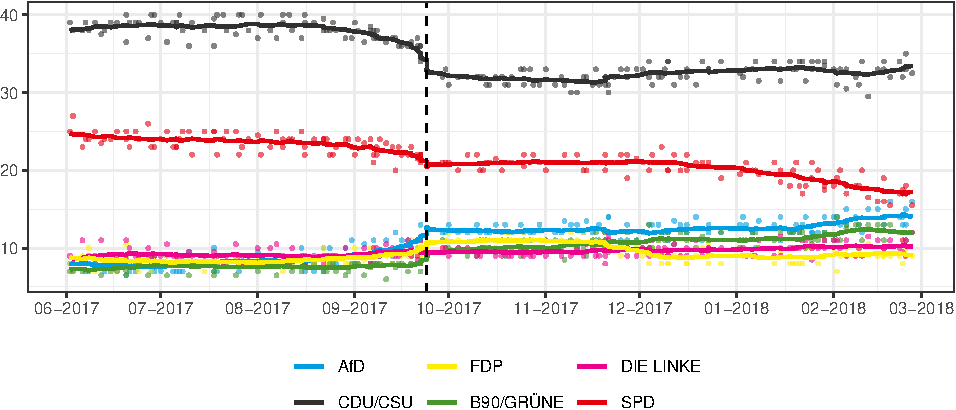
\includegraphics[width=0.6\linewidth]{main_text_files/figure-latex/election polls-1} 

}

\caption{Election polls \label{fig:election_polls}}\label{fig:election polls}
\end{figure}

\hypertarget{german-online-news-market}{%
\subsection{German online news market}\label{german-online-news-market}}

The analysis performed in this paper is based on the news articles of
the following news websites: Bild.de, DIE WELT, FOCUS ONLINE,
Handelsblatt.com, SPIEGEL ONLINE, stern.de, ZEIT ONLINE. As can be seen
from \autoref{fig:news_market}(a), expect for Handelsbaltt.com (position
53), these media outlets are among the top 30 German online news
providers in the period under review in terms of visits.\footnote{The
  term visit is used to describe the call to a website by a visitor. The
  visit begins as soon as a user generates a page impression (PI) within
  an offer and each additional PI, which the user generates within the
  offer, belongs to this visit.}

The main source of income for these privately managed media houses is
digital advertising, even though paid content is playing an increasingly
important role. However, according to a survey on digital news by the
Reuters Institute (Newman et al.
\protect\hyperlink{ref-newman_reuters_2018}{2018}) only 8\% of
respondents pay for online news. The online survey for German data was
undertaken between 19th - 22nd January 2018 by the Hans Bredow
Institute\footnote{\url{https://www.hans-bredow-institut.de/de/projekte/reuters-institute-digital-news-survey}}
with a total sample size of 2038 adults (aged 18+) who access news once
a month or more. Among other questions, participants were asked which
news sources they use to access news online.\footnote{The exact question
  was: ``Which of the following brands have you used to access news
  online in the last week (via websites, apps, social media, and other
  forms of Internet access)? Please select all that apply.''} The
results displayed in \autoref{fig:news_market}(b) indicate that the
media used for the analysis play a relevant role in their consumption.

\begin{figure}

{\centering 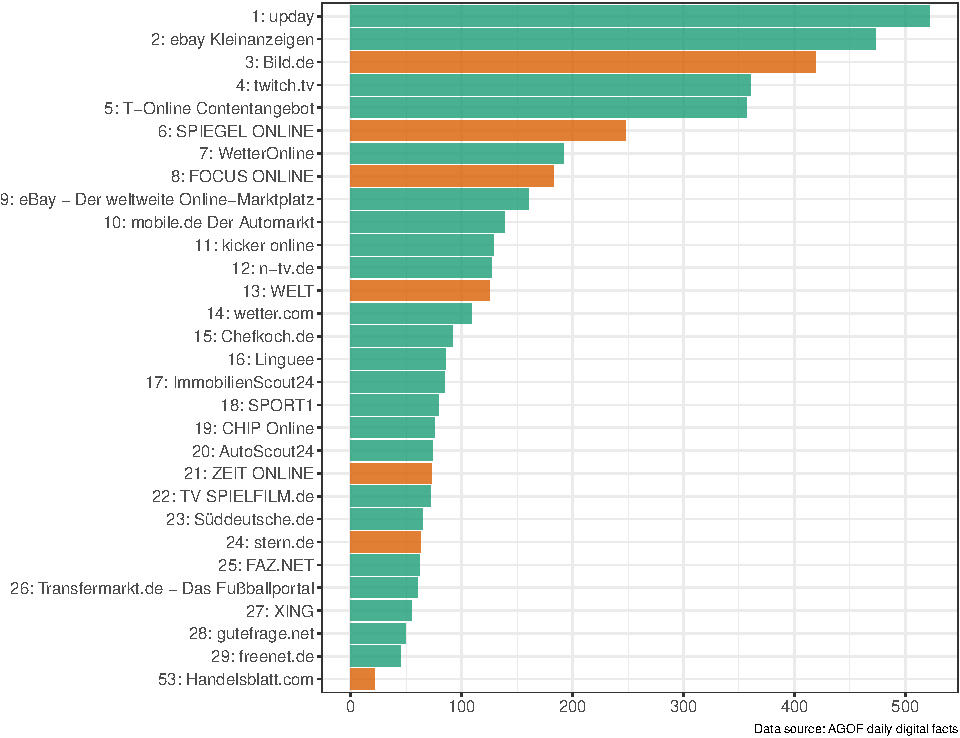
\includegraphics[width=1\linewidth]{main_text_files/figure-latex/unnamed-chunk-1-1} 

}

\caption{Selected german news brands \label{fig:news_market}}\label{fig:unnamed-chunk-1}
\end{figure}

\hypertarget{data}{%
\section{Data}\label{data}}

I conduct the estimation on a sample of 16,473 online news articles from
the seven German news providers mentioned in the previous
section\footnote{Bild.de, DIE WELT, FOCUS ONLINE, SPIEGEL ONLINE,
  stern.de, ZEIT ONLINE, Handelsblatt} about domestic politics and press
releases of the seven parties that have been in the Bundestag since the
2017 federal elections\footnote{CDU, SPD, B90/Grüne, FDP, AfD, Die Linke}.
Both news articles and press releases are dated from June 1, 2017 to
March 1, 2018.

News articles scraped from the Webhose.io API.\footnote{For more
  information see
  \url{https://docs.webhose.io/reference\#about-webhose}. The scraping
  code was written in Python and can be made available on request.} In
order to consider only news about national politics, the articles were
filtered based on their URL.

\autoref{fig:news_distr} shows the distribution of the number of
articles by date and media outlet. There is a high peak around the
federal elections on September, 24th and another one shortly after the
failure of the Jamaica coalition talks on November, 19th (indicated by
the red dotted lines).\footnote{The peak in July especially for
  \emph{stern.de} is due to increased reporting about the G20 summit in
  Hamburg.} Furthermore, \autoref{fig:news_distr} shows that \emph{DIE
WELT} published the most articles on domestic policy, followed by
\emph{stern.de}, \emph{Handelsblatt} and \emph{FOCUS ONLINE}.

\begin{figure}

{\centering 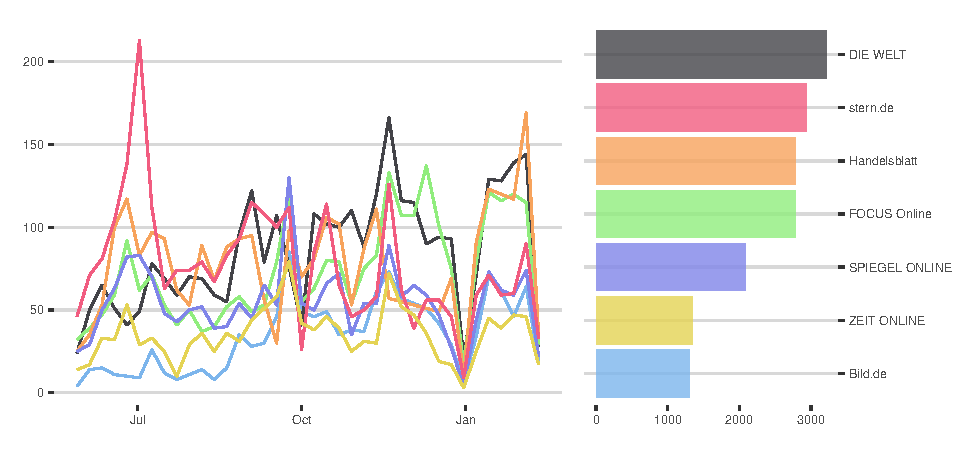
\includegraphics[width=1\linewidth]{main_text_files/figure-latex/news articles-1} 

}

\caption{Distribution of news articles \label{fig:news_distr}}\label{fig:news articles}
\end{figure}

The press releases were scraped from the public websites of the
political parties and parliamentary groups using an automated script
written in \emph{Python}.\footnote{The scraping code was written in
  Python and can be made available on request.}

\begin{figure}

{\centering 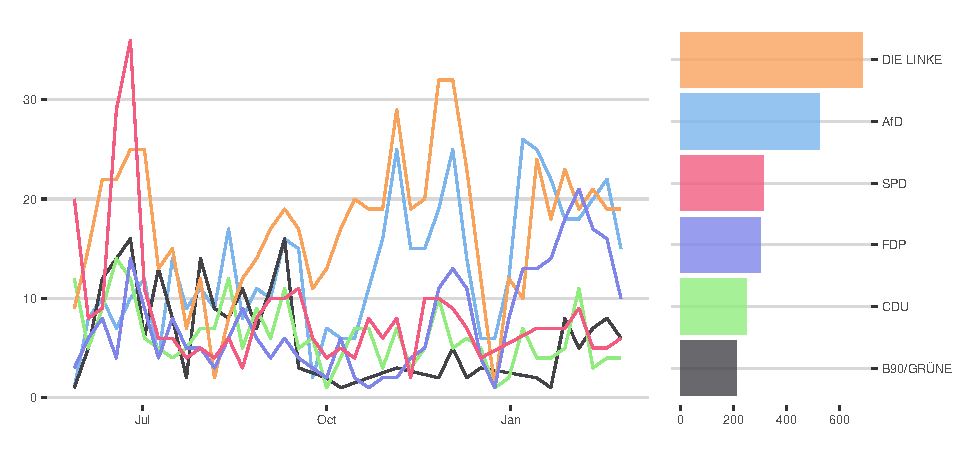
\includegraphics[width=0.9\linewidth]{main_text_files/figure-latex/press releases-1} 

}

\caption{Distribution of press releases \label{fig:press_distr}}\label{fig:press releases}
\end{figure}

Looking at the boxplots of text length (\autoref{fig:text_length}), it
becomes evident that:\footnote{See \autoref{table:text_length} for an
  overview of the summary statistics.}

\begin{itemize}
\tightlist
\item
  mean and median text length of news articles is higher than in press
  releases
\item
  Handelsblatt published new articles with the highest median text
  length (488) followed by ZEIT ONLINE (459), however DIE WELT has the
  article with the highest word count (14.507).
\item
  press releases of CDU have the highest median (256), but also the
  highest standard dev. (106). press releases of FDP have the lowest
  median (144).
\end{itemize}

\begin{figure}

{\centering 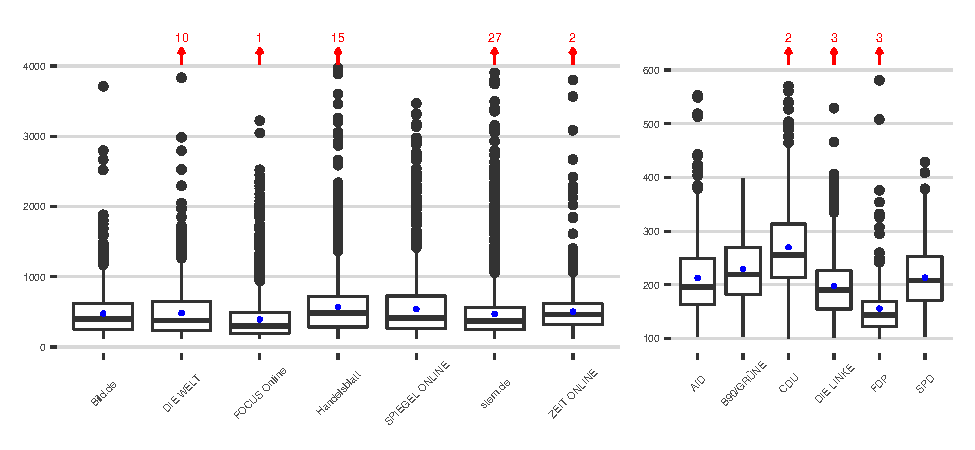
\includegraphics[width=1\linewidth]{main_text_files/figure-latex/text_length-1} 

}

\caption{Text length \label{fig:text_length}}\label{fig:text_length}
\end{figure}

\hypertarget{data-preparation}{%
\subsection{Data preparation}\label{data-preparation}}

To use text as data for statistical analysis, different pre-processing
steps have to be conducted. In fact, in order to use text as data and
reduce the dimensionality to avoid unnecessary computational complexity
and overfitting, pre-processsing the text is a central task in text
mining (Gentzkow, Kelly, and Taddy
\protect\hyperlink{ref-gentzkow_text_2017}{2017}, @bholat\_text\_2015).
Intuitively the term frequency (tf) of a word is a measure of how
important that word may be for the understanding of the text. To
visualize these terms, word clouds are a commonly used technique in text
mining as they translate the tf into the size of the term in the cloud.
As can be seen in \autoref{fig:wordcloud}, problems arise with words
that are highly frequent. For example ``die'', or ``der
(eng.''the``),''und" (eng. ``and''), and ``ist'' (eng. ``is'') are
extremely common but unrelated to the quantity of interest. These terms,
often called stop words (Gentzkow, Kelly, and Taddy
\protect\hyperlink{ref-gentzkow_text_2017}{2017}), are important to the
grammatical structure of a text, but typically don't add any additional
meaning and can therefore be neglected.

\begin{figure}
\centering
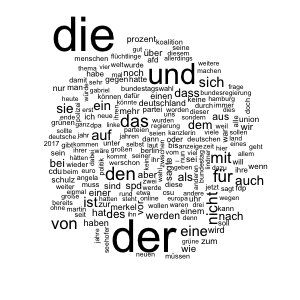
\includegraphics[width=0.4\textwidth,height=\textheight]{../figs/wordcloud.png}
\caption{Wordcloud before pre-processing}
\end{figure}

To remove distorting words, the pre-defined stop word list from the
Snowball project\footnote{\url{http://snowball.tartarus.org/algorithms/german/stop.txt}}
is used together with a customized, domain-specific list of stop-words.
Additionally punctuation character (e.g.~., ,, !, ?, etc.) and all
numbers are removed from the data. A next step to reduce the
dimensionality of text data is to apply an adequate stemming technique.
Stemming is a process by which different morphological variants of a
word are traced back to their common root. For example, ``voting'' and
``vote'' would be treated as two instances of the same token after the
stemming process. There are many different techniques for the stemming
process. I apply the widely used Porter-Stemmer algorithm, which is
based on a set of shortening rules that are applied to a word until it
has a minimum number of syllables.\footnote{\url{https://tartarus.org/martin/PorterStemmer/}}

As an example, the following word clouds represent the most frequent
words of the pre-processed articles for Bild.de and press releases of
AfD. It becomes evident that these are texts discussing domestic policy
issues. The SPD in particular seems to be highly frequent for
\(Bild.de\).

\begin{figure}\centering

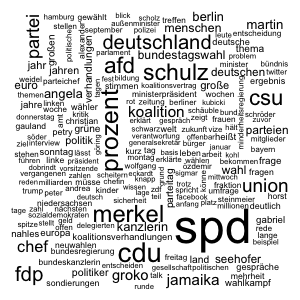
\includegraphics[width=0.4\textwidth,height=\textheight]{../figs/wordcloud_bild.png}
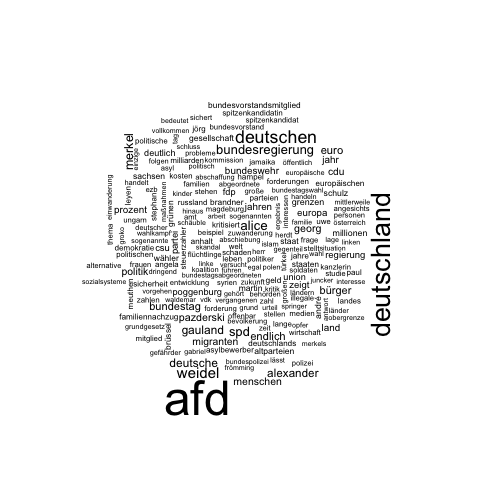
\includegraphics[width=0.4\textwidth,height=\textheight]{../figs/wordcloud_afd.png}

\end{figure}

The next step is to divide the entire data set into individual documents
and to represent these documents as a finite list of unique terms. In
this setting, each news article and each press release represents a
document \(d\), whereby each of these documents can be assigned to a
news website or a party. The sum of all documents forms what is called
the corpus. For each document \(d \in \lbrace 1,...,D \rbrace\) the
number of occurrences of term \(v\) in document \(d\) is computed, in
order to obtain the count \(x_{d,v}\), where each unique term in the
corpus is indexed by some \(v \in \lbrace 1,...,V \rbrace\) and where
\(V\) is the number of unique terms. The \(D\) x \(V\) matrix
\(\boldsymbol{X}\) of all such counts is called the document-term
matrix. Each row in this matrix represents a document, where each entry
in this row counts the occurrences of a unique term in that document.
\autoref{table:dtm} provides a sample output of the document-term matrix
used in this paper, where each document is represented by a unique id
(the row name in the example below). This representation is often
referred to as the bag of words model (Gentzkow, Kelly, and Taddy
\protect\hyperlink{ref-gentzkow_text_2017}{2017}), since the order in
which words are used within a document is disregarded.

\% Table created by stargazer v.5.2.2 by Marek Hlavac, Harvard
University. E-mail: hlavac at fas.harvard.edu \% Date and time: Sun, Jan
03, 2021 - 18:16:10

\begin{table}[!htbp] \centering 
  \caption{Document-term matrix - sample values} 
  \label{table:dtm} 
\begin{tabular}{@{\extracolsep{5pt}} cccccccc} 
\\[-1.8ex]\hline 
\hline \\[-1.8ex] 
 & freude & björn & kurt & familie & grosse & meinungen & familiennachzug \\ 
\hline \\[-1.8ex] 
10777 & $0$ & $0$ & $0$ & $0$ & $0$ & $0$ & $0$ \\ 
8173 & $0$ & $0$ & $0$ & $0$ & $0$ & $0$ & $0$ \\ 
8701 & $0$ & $0$ & $0$ & $0$ & $0$ & $0$ & $0$ \\ 
18632 & $0$ & $0$ & $0$ & $0$ & $0$ & $0$ & $0$ \\ 
13558 & $0$ & $0$ & $0$ & $0$ & $0$ & $0$ & $0$ \\ 
15582 & $0$ & $0$ & $0$ & $0$ & $0$ & $0$ & $0$ \\ 
17177 & $0$ & $0$ & $0$ & $0$ & $0$ & $0$ & $0$ \\ 
684 & $0$ & $0$ & $0$ & $0$ & $0$ & $0$ & $1$ \\ 
14784 & $0$ & $0$ & $0$ & $0$ & $0$ & $0$ & $0$ \\ 
18126 & $0$ & $0$ & $0$ & $0$ & $0$ & $0$ & $0$ \\ 
\hline \\[-1.8ex] 
\end{tabular} 
\end{table}

\hypertarget{estimate-topic-similarity-of-documents}{%
\section{Estimate topic similarity of
documents}\label{estimate-topic-similarity-of-documents}}

\hypertarget{a-structural-topic-model-to-identify-the-latent-topics}{%
\subsection{A structural topic model to identify the latent
topics}\label{a-structural-topic-model-to-identify-the-latent-topics}}

To discover the latent topics in the corpus of press releases and news
articles, a structural topic modeling (STM) developed by (M. E. Roberts,
Stewart, and Airoldi \protect\hyperlink{ref-roberts_model_2016}{2016})
is applied. In general, topic models formalize the idea that documents
are formed by hidden variables (topics) that generate correlations among
observed terms. They belong to the group of unsupervised generative
models, meaning that the true attributes (topics) cannot be observed.
The STM developed by (M. E. Roberts, Stewart, and Airoldi
\protect\hyperlink{ref-roberts_model_2016}{2016}) is a recent extension
of the standard topic modelling technique, labeled as latent Dirichlet
allocation (LDA), which refers to the Bayesian model in (Blei, Ng, and
Jordan \protect\hyperlink{ref-blei_latent_2003}{2003}) that treats each
word in a topic and each topic in a document as generated from a
Dirichlet - distributed prior.\footnote{See also Griffiths and Steyvers
  (\protect\hyperlink{ref-griffiths_probabilistic_2002}{2002}),
  Griffiths and Steyvers
  (\protect\hyperlink{ref-griffiths_finding_2004}{2004}) and Hofmann
  (\protect\hyperlink{ref-hofmann_probabilistic_1999}{1999})}.

The underlying idea for these models suggests that each individual topic
\(k\) potentially contains all of the unique terms within the vocabulary
\(V\) with different probability. Therefore, each topic \(k\) can be
represented as a probability vector \(\phi_k\) over all unique terms
\(V\). Simultaneously, each individual document \(d\) in the corpus can
be represented as a probability distribution \(\theta_d\) over the \(K\)
topics.

The STM is an extension of the LDA process since it allows covariates of
interest (such as the publication date of a document or it's author) to
be included in the prior distributions for both topic proportions
(\(\theta\)) and topic-word distributions (\(\phi\)). This way, STM
offers a method of `structuring' the prior distributions in the topic
model, including additional information in the statistical inference
procedure, while LDA assumes that \(\theta ~ \text{Dirichlet}(\alpha)\)
and \(\phi ~ \text{Dirichlet}(\beta)\), where \(\alpha\) and \(\beta\)
are fitted with the model.

In order to include the covariates in the statistical inference
procedure, two design matrices of covariates (\(X\) and \(Z\)) are
specified, where each row defines a vector of covariates for a specific
document. In \(X\), the covariates for topic prevalence are given, so
that the probability of a topic for each document varies according to
\(X\), rather than resulting from a single common prior. The same
applies to \(Z\), in which the covariates for the word distribution
within a topic are specified. The underlying data generating process to
generate each individual word \(w_{d,n}\) in a document \(d\) for the
\(n^{th}\) word-position can be described as follows:

\begin{itemize}
\tightlist
\item
  for each document \(i\), draw its distribution of topics \(\theta_d\)
  depending on the metadata included in the model defined in \(X\);
\item
  for each topic \(k\), draw its distribution of words \(\phi_k\)
  depending on the metadata included in the model defined in \(Z\);
\item
  for each word \(n\), draw its topic \(z_n\) based on \(\theta_i\);
\item
  for each word word \(n\), draw the term distribution for the selected
  topic \(\phi_{z_{d,n}}\).
\end{itemize}

One crucial assumption to be made for topic models like LDA or STM is
the number of topics (\(K\)) that occur over the entire corpus. There is
not a ``right'' answer to the number of topics that are appropriate for
a given corpus (Grimmer and Stewart
\protect\hyperlink{ref-grimmer_text_2013}{2013}). (M. Roberts, Stewart,
and Tingley
\protect\hyperlink{ref-roberts_stm:_2016}{2016}\protect\hyperlink{ref-roberts_stm:_2016}{b})
propose to measure topic quality through a combination of semantic
coherence and exclusivity of words to topics. Semantic coherence is a
criterion developed by (Mimno et al.
\protect\hyperlink{ref-mimno_optimizing_2011}{2011}) and is closely
related to pointwise mutual information (Newman et al.
\protect\hyperlink{ref-newman_automatic_2010}{2010}): it is maximized
when the most probable words in a given topic frequently co-occur
together.

Using the function \(searchK\) from the \(stm\) package several
automated tests are performed to help choose the number of topics
including the average exclusivity and semantic coherence as well as the
held out likelihood (Wallach, Mimno, and McCallum
\protect\hyperlink{ref-wallach_rethinking_2009}{2009}) and the residuals
(Taddy \protect\hyperlink{ref-taddy_estimation_2012}{2012}). This
process revealed that a model with 40 topics best reflects the structure
in the corpus. Furthermore, I use the author and bi-week dummies of a
document as topical prevalence variable. In other words, I assume that
the probability of a topic to be included in a news article or a press
release depends on the author of that document and when it was
published. I argue that these variables are best suited to capture
temporal and publisher level variation in the documents.

In general inference of mixed-membership models, such as the one applied
in this paper, has been a thread of research in applied statistics
(Blei, Ng, and Jordan \protect\hyperlink{ref-blei_latent_2003}{2003},
@erosheva\_mixed--membership\_2004, @braun\_variational\_2010). Topic
models are usually imprecise as the function to be optimized has
multiple modes, such that the model results can be sensitive to the
starting values (e.g.~the number of topics and the covariates
influencing the prior distributions). Since an ex ante valuation of a
model is hardly possible, I compute a variety of different models and
compare their posterior probability. This enables me to check how
results vary for different model solution (M. Roberts, Stewart, and
Tingley
\protect\hyperlink{ref-roberts_navigating_2016}{2016}\protect\hyperlink{ref-roberts_navigating_2016}{a}).
I then cross-checked some subset of assigned topic distributions to
evaluate whether the estimates align with the concept of interest
(Gentzkow, Kelly, and Taddy
\protect\hyperlink{ref-gentzkow_text_2017}{2017}). These manual audits
are applied together with numeric optimization based on the topic
coherence measure suggested by (Mimno et al.
\protect\hyperlink{ref-mimno_optimizing_2011}{2011}).

\begin{verbatim}
## stm(documents = news_df_sparse, K = 40, prevalence = ~source + 
##     s(year_biweek), data = covariates, init.type = "Spectral")
\end{verbatim}

\hypertarget{results-of-the-stm}{%
\subsection{Results of the STM}\label{results-of-the-stm}}

As stated above, the generative process of the STM results in a topic
distribution \(\theta_d\) for each document \(d\) over all topics \(k\).
The average of each topic across all documents results in the expected
probability of a topic across the whole corpus.
\autoref{fig:topic_distribution} displays the top 20 topics ordered by
their average probability over the whole corpus. Since every topic is a
probability distribution over words, top words may help to understand
what each topic is about and are used as labels in
\autoref{fig:topic_distribution}.\footnote{\autoref{table:top_terms}
  gives an overview of the most probable terms for each topic.} However,
since those most probable words not not necessarily the most exclusive
words and they only represent represent a small fraction of the
probability distribution, interpretation should be done very cautiously.

\begin{itemize}
\tightlist
\item
  1: Topic 35 is the most common topic across the corpus
\item
  4: topic 38 about refugees
\item
  5: topic 39 about the jamaica coalition
\item
  6: followed by topic 8 about the ``GroKo''
\end{itemize}

\begin{figure}

{\centering \includegraphics[width=0.6\linewidth]{main_text_files/figure-latex/Topic distribution-1} 

}

\caption{Top 20 topics by prevalence \label{fig:topic_distribution}}\label{fig:Topic distribution}
\end{figure}

Each document has a probability distribution over all topics, e.g.

\begin{figure}

{\centering 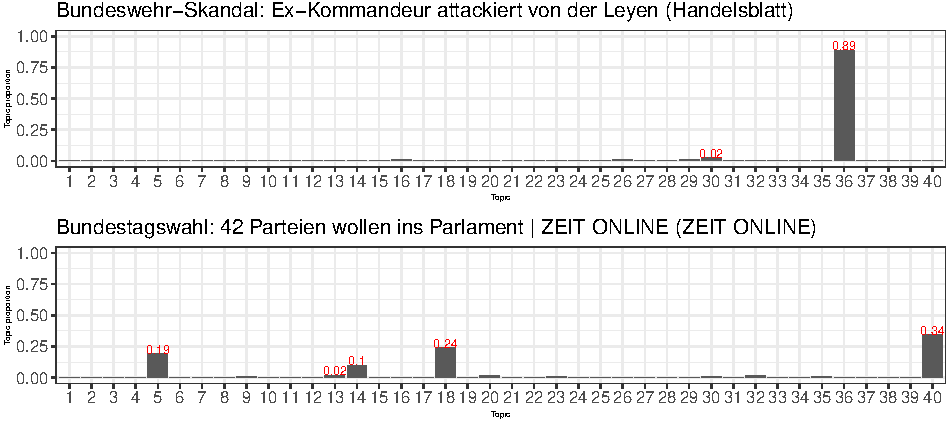
\includegraphics[width=0.8\linewidth]{main_text_files/figure-latex/News articles sample documents-1} 

}

\caption{Topic probability of sample news articles \label{fig:sample_docs12}}\label{fig:News articles sample documents}
\end{figure}

\begin{figure}

{\centering 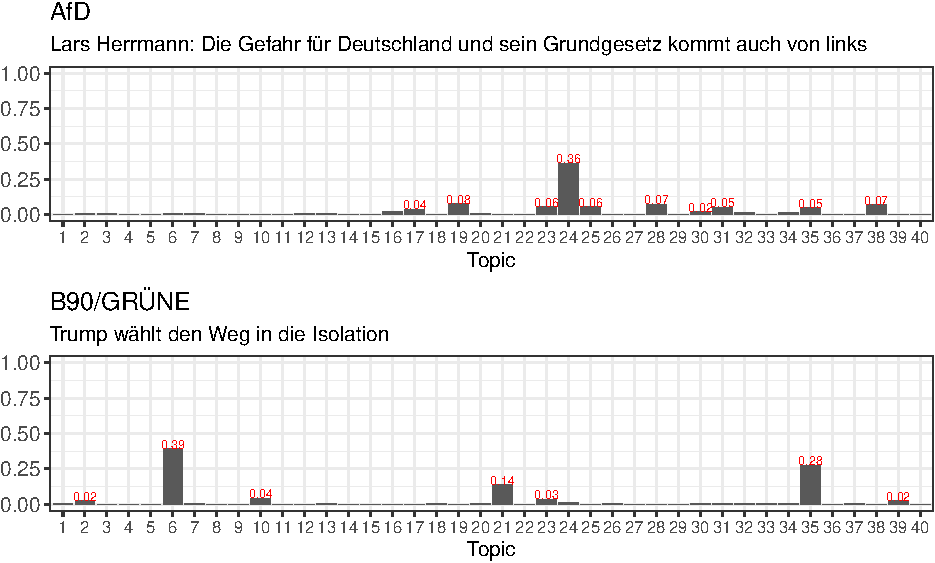
\includegraphics[width=0.8\linewidth]{main_text_files/figure-latex/Press releases sample documents-1} 

}

\caption{Topic probability of sample press releases \label{fig:sample_docs34}}\label{fig:Press releases sample documents}
\end{figure}

\hypertarget{document-cosine-similarity}{%
\subsection{Document Cosine
similarity}\label{document-cosine-similarity}}

Cosine similarity is built on the geometric definition of the dot
product of two vectors. It is a measure for the distance between two
vectors and is defined between zero and one; values towards 1 indicate
similarity.

\[
\text{cosine similarity} = \text{cos}(\theta)=\frac{a*b}{||a|| ||b||}
\] As topic proportions per document are vectors of the same length, the
cosine similarity allows a comparison of the topic distribution between
two documents.\footnote{For applications of cosine similarity to compare
  of topic model outcomes see e.g.~Rehs
  (\protect\hyperlink{ref-rehs_structural_2020}{2020}) and Ramage,
  Dumais, and Liebling
  (\protect\hyperlink{ref-ramage_characterizing_2010}{2010})}

\hypertarget{linear-regression-model}{%
\section{Linear regression model}\label{linear-regression-model}}

\hypertarget{ols-dummy-regression}{%
\subsection{OLS dummy regression}\label{ols-dummy-regression}}

\[
\text{CosineSimilarity}_{i}=\beta_0+\beta_nDn_{j}+\epsilon_i
\]

where the \(D2_{j}, D3_{j}, ... ,Dn_{j}\) represent dummy variables for
a political party \(j\)

\hypertarget{regression-discontinuity-model}{%
\subsection{Regression discontinuity
model}\label{regression-discontinuity-model}}

The idea of regression regression discontinuity design is to use
observations with a \(W_i\) close to \(c\) for the estimation of
\(\beta_1\). \(\beta_1\) is the average treatment effect for
observations with \(W_i = c\) which is assumed to be a good
approximation to the overall treatment effect. In other words,
\(\beta_1\) gives us the average change of news coverage of media outlet
\(i\) after the election day. Since interaction terms \(T_iDn_{j}\) are
included, we can estimate the treatment effect for each party.

Calculate a regression discontinuity model for each newspaper \(i\).

\[
\text{CosineSimilarity}_{i}=\beta_0+\beta_1T_i+\beta_2W_{centered}+\beta_nDn_{j}+\beta_{n+n}T_iDn_{j}+\epsilon_i
\]

where \(D2_{j}, D3_{j}, ... ,Dn_{j}\) represent dummy variables for a
political party \(j\) and \$W\_\{centered\} = \$ date - election day.

\[
T_i = 1 \text{ if date } >= \text{election date} \\
T_i = 0 \text{ if date } < \text{election date}
\]

so that the receipt of treatment \(T_i\) is determined by the threshold
\(c\) (election day) of the continuous variable \(W_i\) (date), the so
called running variable.

\hypertarget{without-interaction-terms}{%
\subsubsection{Without interaction
terms}\label{without-interaction-terms}}

\[
\text{CosineSimilarity}_{i}=\beta_0+\beta_1T_i+\beta_nDn_{j}+\epsilon_i
\]

\hypertarget{with-interaction-terms}{%
\subsubsection{With interaction terms}\label{with-interaction-terms}}

\[
\text{CosineSimilarity}_{i}=\beta_0+\beta_1T_i+\beta_2Dn_{j}+\beta_3T_iDn_{j}+\epsilon_i
\]

The interaction term \(T_i*Dn\) means that the slope can vary on either
side of the treatment threshold for each party.

\begin{itemize}
\tightlist
\item
  The coefficient \(\beta_1\) is how the intercept jumps (the RDD
  effect)
\item
  \(\beta_3\) is how the slope changes for each party
\end{itemize}

\hypertarget{annex}{%
\section{Annex}\label{annex}}

\begin{longtable}[]{@{}lll@{}}
\caption{Online sources for press releases
\label{table:press_releases_sources}}\tabularnewline
\toprule
& Party & Parliamentary Group\tabularnewline
\midrule
\endfirsthead
\toprule
& Party & Parliamentary Group\tabularnewline
\midrule
\endhead
CDU & cdu.de & presseportal.de\tabularnewline
SPD & spd.de & spdfraktion.de\tabularnewline
FDP & fdp.de & fdpbt.de\tabularnewline
B90/Die Grünen & gruene.de & gruene-bundestag.de\tabularnewline
DIE LINKE & die-linke.de &
die-linke.de/start/presse/aus-dem-bundestag\tabularnewline
AfD & afd.de & afdbundestag.de\tabularnewline
\bottomrule
\end{longtable}

\begin{table}[!htbp] \centering 
  \caption{Summary statistics of text length} 
  \label{table:text_length} 
\begin{tabular}{@{\extracolsep{5pt}} ccccccc} 
\\[-1.8ex]\hline 
\hline \\[-1.8ex] 
source & n & mean & sd & median & min & max \\ 
\hline \\[-1.8ex] 
AfD & 523 & 212.83 & 72.16 & 196 & 103 & 553 \\ 
B90/GRÜNE & 211 & 229.32 & 63.37 & 219 & 104 & 399 \\ 
Bild.de & 1303 & 476.07 & 318.28 & 398 & 121 & 3710 \\ 
CDU & 248 & 274.54 & 106.08 & 256 & 100 & 1030 \\ 
DIE LINKE & 686 & 200.47 & 71.78 & 190 & 101 & 1048 \\ 
DIE WELT & 3222 & 509.57 & 612.06 & 380 & 121 & 14507 \\ 
FDP & 301 & 161.9 & 83.78 & 144 & 100 & 999 \\ 
FOCUS Online & 2780 & 393.89 & 317.05 & 297.5 & 121 & 5647 \\ 
Handelsblatt & 2785 & 589.51 & 495.82 & 488 & 121 & 6899 \\ 
SPD & 315 & 213.41 & 56.16 & 208 & 103 & 429 \\ 
SPIEGEL ONLINE & 2089 & 539.09 & 415.05 & 413 & 121 & 3466 \\ 
stern.de & 2943 & 514.66 & 616.55 & 373 & 121 & 9287 \\ 
ZEIT ONLINE & 1351 & 513.75 & 387.14 & 459 & 121 & 8015 \\ 
\hline \\[-1.8ex] 
\end{tabular} 
\end{table}

\% Table created by stargazer v.5.2.2 by Marek Hlavac, Harvard
University. E-mail: hlavac at fas.harvard.edu \% Date and time: Sun, Jan
03, 2021 - 18:16:13

\begin{table}[!htbp] \centering 
  \caption{7 most probable terms per topic} 
  \label{table:top_terms} 
\begin{tabular}{@{\extracolsep{5pt}} cc} 
\\[-1.8ex]\hline 
\hline \\[-1.8ex] 
 & Top Terms \\ 
\hline \\[-1.8ex] 
1 & a, the, s, of, u, brexit, großbritannien \\ 
2 & merkel, angela, kanzlerin, bundeskanzlerin, cdu, merkels, deutschland \\ 
3 & spd, union, cdu, csu, koalitionsvertrag, koalitionsverhandlungen, schulz \\ 
4 & afd, weidel, gauland, alice, alexander, politiker, äußerungen \\ 
5 & stimmen, wahlkreis, kandidaten, afd, wahl, gewählt, fdp \\ 
6 & trump, us, usa, deutschland, präsident, donald, berlin \\ 
7 & cdu, union, peter, politiker, spahn, altmaier, schäuble \\ 
8 & spd, koalition, union, groko, große, koalitionsverhandlungen, parteitag \\ 
9 & afd, partei, sachsen, gauland, parteien, pazderski, höcke \\ 
10 & diesel, unternehmen, deutschland, autos, deutschen, industrie, fahrverbote \\ 
11 & ge, ten, be, le, ver, lambsdorff, te \\ 
12 & gericht, prozess, urteil, richter, staatsanwaltschaft, verfahren, jahre \\ 
13 & berlin, deutschen, osten, o, tag, jahr, millionen \\ 
14 & august, cdu, spd, prozent, bundestagswahl, wahl, parteien \\ 
15 & kohl, helmut, kohls, einheit, kanzler, tod, deutschen \\ 
16 & spd, nahles, andrea, partei, scholz, schulz, schwesig \\ 
17 & csu, seehofer, horst, söder, obergrenze, bayern, chef \\ 
18 & prozent, umfrage, spd, union, fdp, cdu, afd \\ 
19 & polizei, stadt, menschen, polizisten, täter, verletzt, angaben \\ 
20 & euro, milliarden, jahr, millionen, prozent, bund, geld \\ 
21 & grünen, linke, linken, özdemir, partei, wagenknecht, göring \\ 
22 & cdu, niedersachsen, spd, grünen, rot, fdp, landtag \\ 
23 & welt, politik, menschen, jahren, lange, frage, fragen \\ 
24 & g, hamburg, gipfel, polizei, hamburger, demonstranten, scholz \\ 
25 & deutschland, is, verfassungsschutz, syrien, gefährder, islamisten, staat \\ 
26 & steinmeier, schmidt, russland, frank, bundespräsident, glyphosat, walter \\ 
27 & afd, petry, partei, fraktion, frauke, meuthen, gauland \\ 
28 & berliner, berlin, amri, maizière, innenminister, behörden, daten \\ 
29 & gabriel, sigmar, außenminister, spd, schröder, amt, gerhard \\ 
30 & bundestag, spd, abgeordneten, abgeordnete, parlament, abstimmung, fraktion \\ 
31 & türkei, erdogan, türkischen, deutschland, bundesregierung, türkische, deutsche \\ 
32 & frauen, deutschland, kinder, studie, eltern, muslime, antisemitismus \\ 
33 & fdp, jamaika, lindner, koalition, neuwahlen, spd, grünen \\ 
34 & facebook, maas, twitter, gesetz, internet, netz, heiko \\ 
35 & eu, deutschland, europa, bundesregierung, europäischen, deutschen, menschen \\ 
36 & bundeswehr, soldaten, leyen, nato, ursula, einsatz, verteidigungsministerin \\ 
37 & schulz, spd, martin, kanzlerkandidat, wahlkampf, bundestagswahl, partei \\ 
38 & flüchtlinge, deutschland, menschen, zahl, flüchtlingen, familiennachzug, jahr \\ 
39 & fdp, grünen, jamaika, csu, union, grüne, cdu \\ 
40 & bundestagswahl, afd, wahl, prozent, partei, bundestag, parteien \\ 
\hline \\[-1.8ex] 
\end{tabular} 
\end{table}

\hypertarget{references}{%
\section*{References}\label{references}}
\addcontentsline{toc}{section}{References}

\hypertarget{refs}{}
\leavevmode\hypertarget{ref-bholat_text_2015}{}%
Bholat, David M., Stephen Hansen, Pedro M. Santos, and Cheryl
Schonhardt-Bailey. 2015. ``Text Mining for Central Banks.'' \emph{SSRN
Electronic Journal}, June.
\url{http://www.academia.edu/13430482/Text_mining_for_central_banks}.

\leavevmode\hypertarget{ref-blassnig_hitting_2019}{}%
Blassnig, Sina, Sven Engesser, Nicole Ernst, and Frank Esser. 2019.
``Hitting a Nerve: Populist News Articles Lead to More Frequent and More
Populist Reader Comments.'' \emph{Political Communication}, August,
1--23. \url{https://doi.org/10.1080/10584609.2019.1637980}.

\leavevmode\hypertarget{ref-blei_latent_2003}{}%
Blei, David M., Andrew Y Ng, and Michael I Jordan. 2003. ``Latent
Dirichlet Allocation.'' \emph{Journal of Machine Learning Research} 3
(January): 993--1022.

\leavevmode\hypertarget{ref-braun_variational_2010}{}%
Braun, Michael, and Jon McAuliffe. 2010. ``Variational Inference for
Large-Scale Models of Discrete Choice.'' \emph{Journal of the American
Statistical Association} 105 (489): 324--35.
\url{https://doi.org/10.1198/jasa.2009.tm08030}.

\leavevmode\hypertarget{ref-dewenter_einfuhrung_2014}{}%
Dewenter, Ralf, and Jürgen Rösch. 2014. \emph{Einführung in die neue
Ökonomie der Medienmärkte: Eine wettbewerbsökonomische Betrachtung aus
Sicht der Theorie der zweiseitigen Märkte}. Springer-Verlag.

\leavevmode\hypertarget{ref-druckman_impact_2005}{}%
Druckman, James N., and Michael Parkin. 2005. ``The Impact of Media
Bias: How Editorial Slant Affects Voters.'' \emph{The Journal of
Politics} 67 (4): 1030--49.
\url{https://doi.org/10.1111/j.1468-2508.2005.00349.x}.

\leavevmode\hypertarget{ref-eberl_lying_2018}{}%
Eberl, Jakob-Moritz. 2018. ``Lying Press: Three Levels of Perceived
Media Bias and Their Relationship with Political Preferences.''
\emph{Communications}, March.
\url{https://doi.org/10.1515/commun-2018-0002}.

\leavevmode\hypertarget{ref-eberl_one_2017}{}%
Eberl, Jakob-Moritz, Hajo G. Boomgaarden, and Markus Wagner. 2017. ``One
Bias Fits All? Three Types of Media Bias and Their Effects on Party
Preferences.'' \emph{Communication Research} 44 (8): 1125--48.
\url{https://doi.org/10.1177/0093650215614364}.

\leavevmode\hypertarget{ref-erosheva_mixed-membership_2004}{}%
Erosheva, Elena, Stephen Fienberg, and John Lafferty. 2004.
``Mixed-Membership Models of Scientific Publications.''
\emph{Proceedings of the National Academy of Sciences} 101 (suppl 1):
5220--7. \url{https://doi.org/10.1073/pnas.0307760101}.

\leavevmode\hypertarget{ref-gentzkow_media_2004}{}%
Gentzkow, Matthew A., and Jesse M. Shapiro. 2004. ``Media, Education and
Anti-Americanism in the Muslim World.'' \emph{Journal of Economic
Perspectives} 18 (3): 117--33.
\url{https://doi.org/10.1257/0895330042162313}.

\leavevmode\hypertarget{ref-gentzkow_text_2017}{}%
Gentzkow, Matthew, Bryan T. Kelly, and Matt Taddy. 2017. ``Text as
Data.'' Working Paper 23276. National Bureau of Economic Research.
\url{https://doi.org/10.3386/w23276}.

\leavevmode\hypertarget{ref-griffiths_probabilistic_2002}{}%
Griffiths, Thomas L., and Mark Steyvers. 2002. ``A Probabilistic
Approach to Semantic Representation.'' \emph{Proceedings of the Annual
Meeting of the Cognitive Science Society} 24 (24).
\url{https://escholarship.org/uc/item/44x9v7m7}.

\leavevmode\hypertarget{ref-griffiths_finding_2004}{}%
---------. 2004. ``Finding Scientific Topics.'' \emph{Proceedings of the
National Academy of Sciences} 101 (suppl 1): 5228--35.
\url{https://doi.org/10.1073/pnas.0307752101}.

\leavevmode\hypertarget{ref-grimmer_text_2013}{}%
Grimmer, Justin, and Brandon Stewart. 2013. ``Text as Data: The Promise
and Pitfalls of Automatic Content Analysis Methods for Political
Texts.'' \emph{Political Analysis} 21: 267--97.

\leavevmode\hypertarget{ref-groseclose_measure_2005}{}%
Groseclose, Tim, and Jeffrey Milyo. 2005. ``A Measure of Media Bias.''
\emph{The Quarterly Journal of Economics} 120 (4): 1191--1237.
\url{https://www.jstor.org/stable/25098770}.

\leavevmode\hypertarget{ref-hofmann_probabilistic_1999}{}%
Hofmann, Thomas. 1999. ``Probabilistic Latent Semantic Indexing.'' In
\emph{Proceedings of the 22Nd Annual International ACM SIGIR Conference
on Research and Development in Information Retrieval}, 50--57. SIGIR
'99. New York, NY, USA: ACM.
\url{https://doi.org/10.1145/312624.312649}.

\leavevmode\hypertarget{ref-kepplinger_einfluss_2004}{}%
Kepplinger, Hans Mathias, and Marcus Maurer. 2004. ``Der Einfluss Der
Pressemitteilungen Der Bundesparteien Auf Die Berichterstattung Im
Bundestagswahlkampf 2002.'' In \emph{Quo Vadis Public Relations? Auf Dem
Weg Zum Kommunikationsmanagement: Bestandsaufnahmen Und Entwicklungen},
edited by Juliana Raupp and Joachim Klewes, 113--24. Wiesbaden: VS
Verlag für Sozialwissenschaften.
\url{https://doi.org/10.1007/978-3-322-83381-5_9}.

\leavevmode\hypertarget{ref-lott_is_2014}{}%
Lott, John R., and Kevin A. Hassett. 2014. ``Is Newspaper Coverage of
Economic Events Politically Biased?'' \emph{Public Choice} 160 (1):
65--108. \url{https://doi.org/10.1007/s11127-014-0171-5}.

\leavevmode\hypertarget{ref-mimno_optimizing_2011}{}%
Mimno, David, Hanna M. Wallach, Edmund Talley, Miriam Leenders, and
Andrew McCallum. 2011. ``Optimizing Semantic Coherence in Topic
Models.'' In \emph{Proceedings of the Conference on Empirical Methods in
Natural Language Processing}, 262--72. EMNLP '11. Stroudsburg, PA, USA:
Association for Computational Linguistics.
\url{http://dl.acm.org/citation.cfm?id=2145432.2145462}.

\leavevmode\hypertarget{ref-newman_automatic_2010}{}%
Newman, David, Jey Han Lau, Karl Grieser, and Timothy Baldwin. 2010.
``Automatic Evaluation of Topic Coherence.'' In \emph{Human Language
Technologies: The 2010 Annual Conference of the North American Chapter
of the Association for Computational Linguistics}, 100--108. HLT '10.
Stroudsburg, PA, USA: Association for Computational Linguistics.
\url{http://dl.acm.org/citation.cfm?id=1857999.1858011}.

\leavevmode\hypertarget{ref-newman_reuters_2018}{}%
Newman, Nic, Richard Fletcher, Antonis Kalogeropoulos, David Levy, and
Rasmus Kleis Nielsen. 2018. ``Reuters Institute Digital News Report
2018.'' Reuters Institute for the Study of Journalism.
\url{http://media.digitalnewsreport.org/wp-content/uploads/2018/06/digital-news-report-2018.pdf?x89475}.

\leavevmode\hypertarget{ref-ramage_characterizing_2010}{}%
Ramage, Daniel, Susan Dumais, and Daniel Liebling. 2010.
\emph{Characterizing Microblogs with Topic Models}.

\leavevmode\hypertarget{ref-rehs_structural_2020}{}%
Rehs, Andreas. 2020. ``A Structural Topic Model Approach to Scientific
Reorientation of Economics and Chemistry After German Reunification.''
\emph{Scientometrics} 125 (2): 1229--51.
\url{https://doi.org/10.1007/s11192-020-03640-0}.

\leavevmode\hypertarget{ref-roberts_model_2016}{}%
Roberts, Margaret E., Brandon M. Stewart, and Edoardo M. Airoldi. 2016.
``A Model of Text for Experimentation in the Social Sciences.''
\emph{Journal of the American Statistical Association} 111 (515):
988--1003. \url{https://doi.org/10.1080/01621459.2016.1141684}.

\leavevmode\hypertarget{ref-roberts_navigating_2016}{}%
Roberts, Margaret, Brandon Stewart, and Dustin Tingley. 2016a.
``Navigating the Local Modes of Big Data: The Case of Topic Models.'' In
\emph{Computational Social Science: Discovery and Prediction}. New York:
Cambridge University Press.

\leavevmode\hypertarget{ref-roberts_stm:_2016}{}%
---------. 2016b. ``Stm: R Package for Structural Topic Models.''
\emph{Journal of Statistical Software} forthcoming (December).

\leavevmode\hypertarget{ref-stromback_four_2008}{}%
Strömbäck, Jesper. 2008. ``Four Phases of Mediatization: An Analysis of
the Mediatization of Politics.'' \emph{The International Journal of
Press/Politics} 13 (3): 228--46.
\url{https://doi.org/10.1177/1940161208319097}.

\leavevmode\hypertarget{ref-taddy_estimation_2012}{}%
Taddy, Matt. 2012. ``On Estimation and Selection for Topic Models.'' In
\emph{Proceedings of the 15th International Conference on Artificial
Intelligence and Statistics}.

\leavevmode\hypertarget{ref-takens_media_2013}{}%
Takens, Janet, Wouter Atteveldt, Anita van Hoof, and Jan Kleinnijenhuis.
2013. ``Media Logic in Election Campaign Coverage.'' \emph{European
Journal of Communication} 28 (June): 277--93.
\url{https://doi.org/10.1177/0267323113478522}.

\leavevmode\hypertarget{ref-wallach_rethinking_2009}{}%
Wallach, Hanna M., David M. Mimno, and Andrew McCallum. 2009.
``Rethinking LDA: Why Priors Matter.'' In \emph{Advances in Neural
Information Processing Systems 22}, edited by Y. Bengio, D. Schuurmans,
J. D. Lafferty, C. K. I. Williams, and A. Culotta, 1973--81. Curran
Associates, Inc.
\url{http://papers.nips.cc/paper/3854-rethinking-lda-why-priors-matter.pdf}.

\end{document}
